\documentclass[english, 12pt, a4paper, sci, utf8, a-1b, online]{aaltothesis}

\usepackage{graphicx}

\usepackage{amsfonts, amssymb, amsbsy, amsmath}
\usepackage[english, finnish]{babel}
\usepackage{natbib}

\usepackage{csvsimple}

\newpage

\bibliographystyle{plainnat}
\setcitestyle{authoryear,open={(},close={)}}


%\thesistitle{Bayesian model validation merics in retail datasets}

\degreeprogram{Engineering Physics and Mathematics}

\major{Mathematics and Systems Sciences}

\code{SCI3029}

\univdegree{BSc}


\thesisauthor{Leevi Rönty}

\thesistitle{Bayesian model validation metrics in retail datasets}
%\thesistitle[Opinnäytteen otsikko]{Opinnäyteen\\ otsikko}
%%

%%
\place{Espoo}
%%



\date{14.10.2020}

\supervisor{Prof.\ Fabricio Oliveira}

\advisor{DSc\ (Tech.) Mikko Ervasti}
\advisor{DSc\ (Tech.) Paavo Niskala} % TODO: checkaa voiko tähän lisätä kahta näin

\uselogo{aaltoBlue}{''}


\keywords{Bayesian models\spc model validation\spc
	information criterion\spc Facebook Prophet}

\thesisabstract{
Tiivistelmässä on lyhyt selvitys kirjoituksen tärkeimmästä sisällöstä: mitä ja
miten on tutkittu, sekä mitä tuloksia on saatu. Tämän opinnäytteen 
tiivistelmäteksti kirjoitetaan opinnäytteen luettavan osan
lomakkeen lisäksi myös pdf-tiedoston metadataan. Kirjoita tähän metadataan
kirjoitettavaa teksti. Metadatatekstissa ei saa olla erikoismerkkejä,
rivinvaiho- tai kappaleenjakomerkkiä, joten näitä merkkeja ei saa käyttää tässä.
Jos tiivistelmäsi ei sisällä erikoimerkkejä eikä kaipaa kappaleenjakoa, voit
hyödynttää makroa abstracttext luodessasi lomakkeen tiivistelmää (katso
kommentti alla). Metadatatiivistelmatekstin on muuten oltava sama kuin
lomakkeessa oleva teksti.
}

\copyrighttext{Copyright \noexpand\copyright\ \number\year\ \ThesisAuthor}
{Copyright \copyright{} \number\year{} \ThesisAuthor 
\\\\The document can be stored and made available to the public on the open internet pages of Aalto University.\\
All other rights are reserved.
}


%% Kaikki mikä paperille tulostuu, on tämän jälkeen
\begin{document}

\makecoverpage{}


\makecopyrightpage{}


\begin{abstractpage}[english]
Your abstract in English. Keep the abstract short. The abstract explains your
research topic, the methods you have used, and the results you obtained.
\end{abstractpage}

\newpage


% TODO: Paavo kans mukaan advisoreiksi
\thesistitle{Bayeslaisten mallien validointi vähittäismyynnin aineistoissa}
\degreeprogram{Teknillinen fysiikka ja matematiikka}
\major{Matematiikka ja systeemitieteet}
\advisor{TkT Mikko Ervasti}
\advisor{TkT Paavo Niskala}
\keywords{Bayeslaiset mallit\spc mallin validointi\spc
	informaatiokriteeri\spc Facebook Prophet}

\begin{abstractpage}[finnish]
Tiivistelmässä on lyhyt selvitys kirjoituksen tärkeimmästä sisällöstä: mitä ja
miten on tutkittu, sekä mitä tuloksia on saatu.

Tämän opinnäytteen tiivistelmäteksti kirjoitetaan opinnäytteen luettavan osan 
lomakkeen lisäksi myös pdf-tiedoston metadataan 
$\backslash$thesisabstract-makron avulla (kasto yllä). Kirjoita tähän
luettavaan tiivistelmälomakkeeseen menevä teksti. Tässä saa olla erikoismerkkejä
kuten kreikkalaiset kirjaimet ja rivinvaiho- ja kappaleenjakomerkit. Tämän
tekstin on muuten oltava sama kuin metedatatiivistelmän teksti.

Jos tiivistelmäsi ei sisällä erikoimerkkejä eikä kaipaa kappaleenjakoa, voit
hyödynttää makroa $\backslash$abstracttext luodessasi lomakkeen tiivistelmää
(katso kommentti alla).

\end{abstractpage}

%% Sisällysluettelo
\thesistableofcontents

\cleardoublepage

%% Leipäteksti alkaa
%%
\section{Introduction}

%Modelling and forecasting of sales timeseries helps in deciding marketing investments
%Company (Sellforte) makes lots of forecasts to customers
%Validation of used models is a critical part of the process and a subject of ongoing developement in company
%Cross validation is best practice, but it’s not always feasible to do
%Data from a short time frame or expensive fitting of models
%Information criterions aim to estimate fit to out-of-sample data

%%% Motivaatio ja tausta
%- Yritykset laativat paljon ennusteita
%- Mallien validointi on oleellinen osa prosessia
%- Bayeslaisten mallien validointi on kuitenkin suhteellisen uusi asia


%%% Haasteet ja kirjallisuus
%- Bayeslaisten mallien validoinnin nykytila on "unsatisfactory"
%- Kuhunkin käytetyimmistä menetelmistä liittyy ongelmia
%- Entä jos sakkofunktiona MAPE?

%%% Mitä tehdään
%- Mallinnetaan myyntiä Prophetilla
%- Implementoidaan IC:t prophetille
%- Vertaillaan tuloksia 'ad-hoc' -menetelmiin

%%% Työn rakenne
%- Ei välttis pakollinen

Businesses need to forecast a multitude of things to succeed. As companies collect more and more data 
the possibilities of forecastable subjects and possible features increase dramatically. However, one can't just
thow more features at a model and except it to perform well. Also not all models are suitable for all 
forecasting tasks. The amount of possible models is endless, but most of them are bad. To find the usefull ones
we must be able to measure the goodness of a model.

Model validation is an integral part of a robust modelling framework. Bayesian models are a relatively novel
model type which has gained a lot of populatiry in recent years as computational power of modern computers 
has kept rising. As a relatively new method not too many validation metrics have been proposed with these kinds
of models in mind.

The current state of model validation for bayesian models can be described as "unsatisfactory". Information
criterions which try to predict out of sample fit can have strong biases and some may not take into consideration
the nature of bayesian models and distributions of parameters. Cross validation can be computationally extremely
intensive. Also most information criterions are based on a loss function proportional to the root mean square of errors,
but that may not always be the most usefull function to optimize for. In some businesses the consecuences of errors
in forecasts can be described better with the mean absotule percentage error. All in all there does not
exist a clearly better method for solving all bayesian model validation problems.

In this paper we will model sales timeseries of some Wallmart stores in the United States. We will be using 
the Facebook's Prophet modelling framework. It consists of a flexible bayesian model which can be customized 
to fit a wide range of possible time series modelling tasks. We will implement some information criterions 
for the model and compare it to more ad-hoc methods for model validation. 



%\section{Aikaisempi tutkimus}
\section{Background}

%Tässä osassa selvitetään, mitä tutkimuksen kohteena olevasta aiheesta tiedetään
%entuudestaan. Selvityksen tulee kattaa tasapainoisesti koko tutkimuskenttä. 

%Kun opinnäytetyötä kirjoitetaan, on noudatettava ohjeita, jotka koskevat
%opinnäytteen rakennetta, käytäntöjä, muotoseikkoja sekä ulkoasua. Esitellään
%näitä ohjeita tarkemmin.

%% Osan hienojaottelua alaosiin, eikä välttämättä edes tarpeen, tässä vain
%% esimerkkinä. Käytä harkintasi mukaan osan jaottelua, joskus alaotsikot
%% selventävät asioita ja joskus vain sirpaloittavat tarpeettomasti tekstiä.
%%  Jaottelu menee seuraavasti:
%% \section{osan otsikko} 
%% \subsection{alaotsikko}
%% \subsubsection{ala-alaotsikko}
%% Tätä pitemälle ei pidä jaotella. 
%%
%% Three levels of hierarchy in sectioning should be enough



%Työn tausta:
%– Esitellään, mitä kirjallisuudessa on aiemmin esitetty
%– Formaatti: ”Henkilöt X tutkivat asiaa Y ja tulivat siihen
%johtopäätökseen, että Z”
%– Oman työn kontribuutiota voi tässä osiossa peilata
%kirjallisuuteen, joskin se on syytä pitää taka-alalla
%– Teknistä sanastoa saa käyttää, mutta ei kaavoja tai muuta
%matemaattista notaatiota


% Bayesian models
% - What models are
% - What bayesian models do
% - Why bayesian models


% Model validation
% A survey of Bayesian predictive methods
% for model assessment, selection and
% comparison
% - Vehtarin paperista inspistä
% - Myös point predictive -jutut
% - Kans pivotal quantities
% - ero point predictionin ja muiden välillä


In retail business many things can be a subject for optimizing. Predictions of sales can be used
to minimize waste and ensure sufficient supply of goods. Advertising products can yield greater sales
but not all ads are equally effective. Shifting marketing investments to more impactfull marketing channels
can increase sales while keeping costs the same. Both of these examples demonstrate scenarios where statistical models can be used to
avoid making unoptimal decisions my manual guesswork.

Models can be viewed as simplifications of reality. This means that no model never really mathces the true data generating processes, 
but if we can formulate a model that works well enough we can try to draw some conclusions from them. Most of the models we are concerned with
link together some explanatory variables to the measured data. The parameters of the function are learned by fitting the data to the model.
The fitted model can then be used to predict future observations if we can know the explanatory variables beforehand. The fitted model parameters
can also give insight on the behaviour of the physical world, assuming that said parameters have a sensible interpretation.

Bayesian models differ from frequentist models in two major ways. In bayesian thinking parameters are not expressed as point values but distibutions.
Uncertainty can be expressed with wider distributions. New data is not the sole source of the newly fitted parameters as it is merely used to
update prior beliefs about parameter distribution. 






\subsection{Rakenne}

\section{Tutkimusaineisto ja -menetelmät}

Tässä osassa kuvataan käytetty tutkimusaineisto ja tutkimuksen metodologiset
valinnat, sekä kerrotaan tutkimuksen toteutustapa ja käytetyt menetelmät.


\section{Tulokset}

Tässä osassa esitetään tulokset ja vastataan tutkielman alussa
esitettyihin tutkimuskysymyksiin. Tieteellisen kirjoitelman
arvo mitataan tässä osassa esitettyjen tulosten perusteella. 

%% Huomaa seuraavassa kappaleessa lainausmerkkien ulkopuolella piste, 
%% koska piste ei lopeta lainattua tekstinpätkää.
%% Jos lainattu tekstinpätkä loppuu välimerkkiin, tulee välimerkki
%% lainausmerkkien sisälle: 
%% "Et tu, Brute?" sanoi Caesar kuollessaan.
Tutkimustuloksien merkitystä on aina syytä arvioida ja tarkastella
kriittisesti.  Joskus tarkastelu voi olla tässä osassa, mutta se
voidaan myös jättää viimeiseen osaan, jolloin viimeisen osan nimeksi
tulee >>Tarkastelu>>. Tutkimustulosten merkitystä voi arvioida myös
>>Johtopäätökset>>-otsikon alla viimeisessä osassa. 

Tässä osassa on syytä myös arvioida tutkimustulosten luotettavuutta.
Jos tutkimustulosten merkitystä arvioidaan >>Tarkastelu>>-osassa,
voi luotettavuuden arviointi olla myös siellä. 





%\catcode`\$=12
%\csvautotabular{test_data.csv}
%\catcode`\$=3

\begin{table*}[!ht]
	\csvreader[%
	 tabular={|c|c|c|c|c|c|},
					table head = \hline\textbf{Model} &\textbf{WAIC}\\\hline,
					late after line= \\,
					late after last line=\\\hline %
					]{test.csv}{model_name=\mname,WAIC=\waic}%
					{\mname & \waic}
				 \centering
					\caption{\label{table1}Number by category}
	\end{table*}

%\csvautotabular{../tables/single_store_4_of_A_metrics.csv}




%\section{Yhteenveto}
\section{Summary} 

Opinnäytteen tekijä vastaa siitä, että opinnäyte on tässä dokumentissa
ja opinnäytteen tekemistä käsittelevillä luennoilla sekä
harjoituksissa annettujen ohjeiden mukainen muotoseikoiltaan,
rakenteeltaan ja ulkoasultaan.



%
% LÄHDELUETTELO
%  BibTeX-tiedoston kokoaminen onnistuu näppärästi esim. 
%  Firefoxin Zotero-lisäosalla http://www.zotero.org/
%  joka osaa poimia viitteet suoraan Google Scholarista.
%


% Ladataan library.bib
\bibliography{library}


%% Liitteet
%% Poista a.o. \clearpage- ja \thesisappendix -makrot, jos liiteitä ei ole.
\clearpage
\thesisappendix

\section{Esimerkki liitteestä\label{LiiteA}}

Kaavojen numerointi muodostaa liitteissä oman kokonaisuutensa:
\begin{align}
d \wedge A &= F, \label{liitekaava1}\\
d \wedge F &= 0. \label{liitekaava2}
\end{align}


\clearpage
\section{Toinen esimerkki liitteestä\label{LiiteB}}

%% Liitteiden kaavat, taulukot ja kuvat numeroidaan omana kokonaisuutenaan

Liitteissä voi myös olla kuvia, jotka
eivät sovi leipätekstin joukkoon:
%% Ympäristön figure parametrit htb pakottavat
%% kuvan tähän, eikä LaTeX yritä siirrellä niitä
%% hyväksi katsomaansa paikkaan. 
%% Ympäristöä center voi käyttää \centering-
%% komennon sijaan
%%
\begin{figure}[htb]
\centering
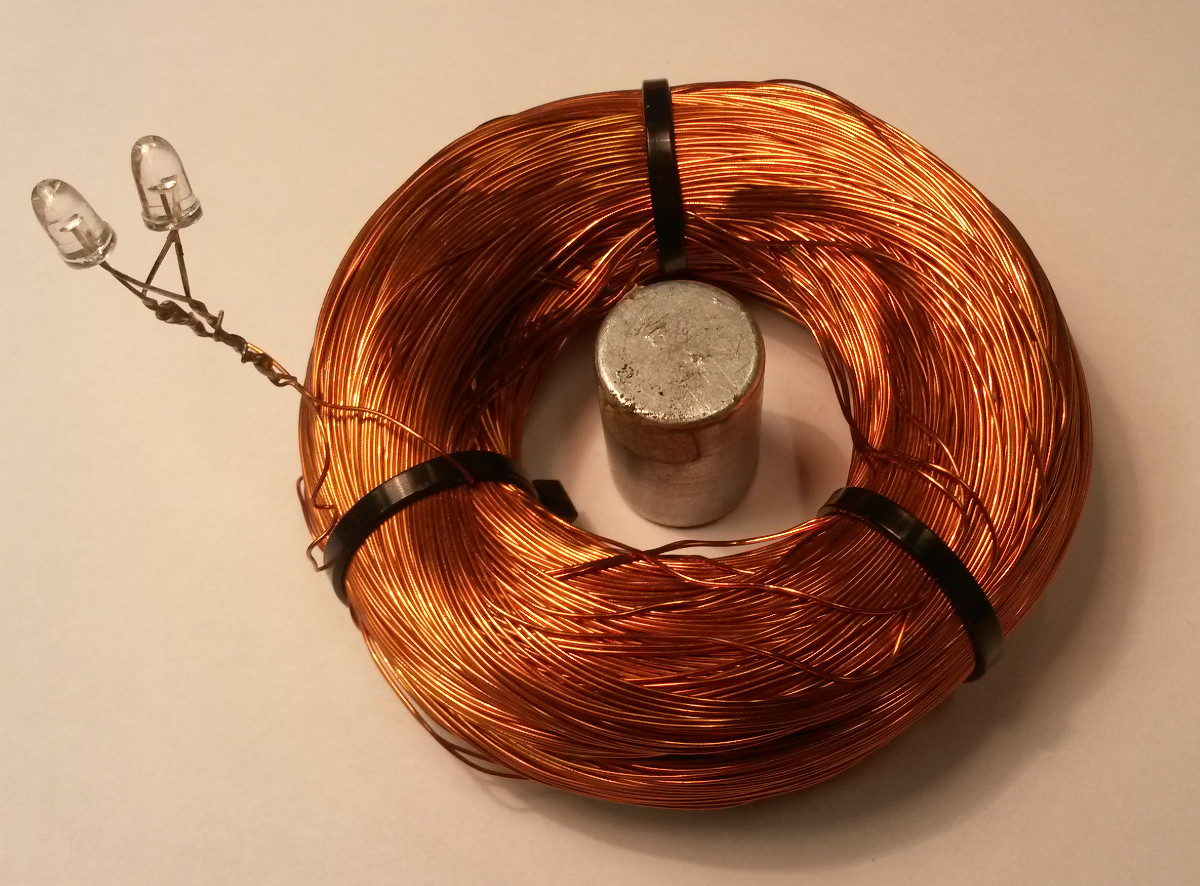
\includegraphics[height=8cm]{./ledspole.jpg}
\caption{Kuvateksti, jossa on liitteen numerointi}
\label{liitekuva}
\end{figure}
%%
Liitteiden taulukoiden numerointi on kuvien ja kaavojen kaltainen:
\begin{table}[htb]
\caption{Taulukon kuvateksti.}
\label{liitetaulukko}
\centering
\fbox{
\begin{tabular}{lp{0.5\linewidth}}
9.00--9.55  & Käytettävyystestauksen tiedotustilaisuus (osanottajat
ovat saaneet sähköpostitse valmistautumistehtävät, joten tiedotustilaisuus
voidaan pitää lyhyenä).\\
9.55--10.00 & Testausalueelle siirtyminen
\end{tabular}}
\end{table}
Kaavojen numerointi muodostaa liitteissä oman kokonaisuutensa:
\begin{align}
T_{ik} &= -p g_{ik} + w u_i u_k + \tau_{ik},  \label{liitekaava3} \\
n_i    &= n u_i + v_i.                      \label{liitekaava4}
\end{align}

\end{document}
